\section{Results}\label{sec:results}

We apply our method to another set of mock data, the spherical models
for the Gaia challenge by Walker and Penarrubia. They consist of
dynamical tracer populations with density distribution

\begin{equation}
\nu_*(r) = \nu_0\left(\frac{r}{r_*}\right)^{-\gamma_*} \left[1+\left(\frac{r}{r_*}\right)^{\alpha_*}\right]^{(\gamma_*-\beta_*)/\alpha_*}
\end{equation}

inside dark matter halos of the form

\begin{equation}
\rho_{\text{DM}} = \rho_0\left(\frac{r}{r_{\text{DM}}}\right)^{-\gamma_{\text{DM}}}\left[1+\left(\frac{r}{r_{\text{DM}}}\right)^{\alpha_{\text{DM}}}\right]^{(\gamma_{\text{DM}}-\beta_{\text{DM}})/\alpha_{\text{DM}}}
\end{equation}

with scale radii $r_*, r_\text{DM}$, inner and outer logarithmic
slopes of $\gamma_*, \gamma_{\text{DM}}$ and
$\beta_*,\beta_{\text{DM}}$, with transition parameters $\alpha_*,
\alpha_{\text{DM}}$.

The anisotropy follows the functional form of \citet{Osipkov1979} and
\citet{Merritt1985},

\begin{equation}
\beta_{\text{anisotropy}}(r)=1-\frac{\sigma_\theta^2}{\sigma_r^2} = \frac{r^2}{r^2+r_a^2}.
\end{equation}

with scale radius $r_a$, turning over from nearly isotropic at $r\to
0$ to radially biased at $r_*=r_a$.

Of these distributions, finite samplings are taken and converted to
mock observational data including spectral indices, systemic
velocities, proper motions, binary motion.


\subsection{Cusps and Cores}

Applied on a profile with a core in the DM density profile, our method
converges fast in the beginning and reproduces the density profile very well after 50000 iterations (fig. \ref{fig:cusp}).

\begin{figure*}
\begin{center}
\hspace{-7mm}
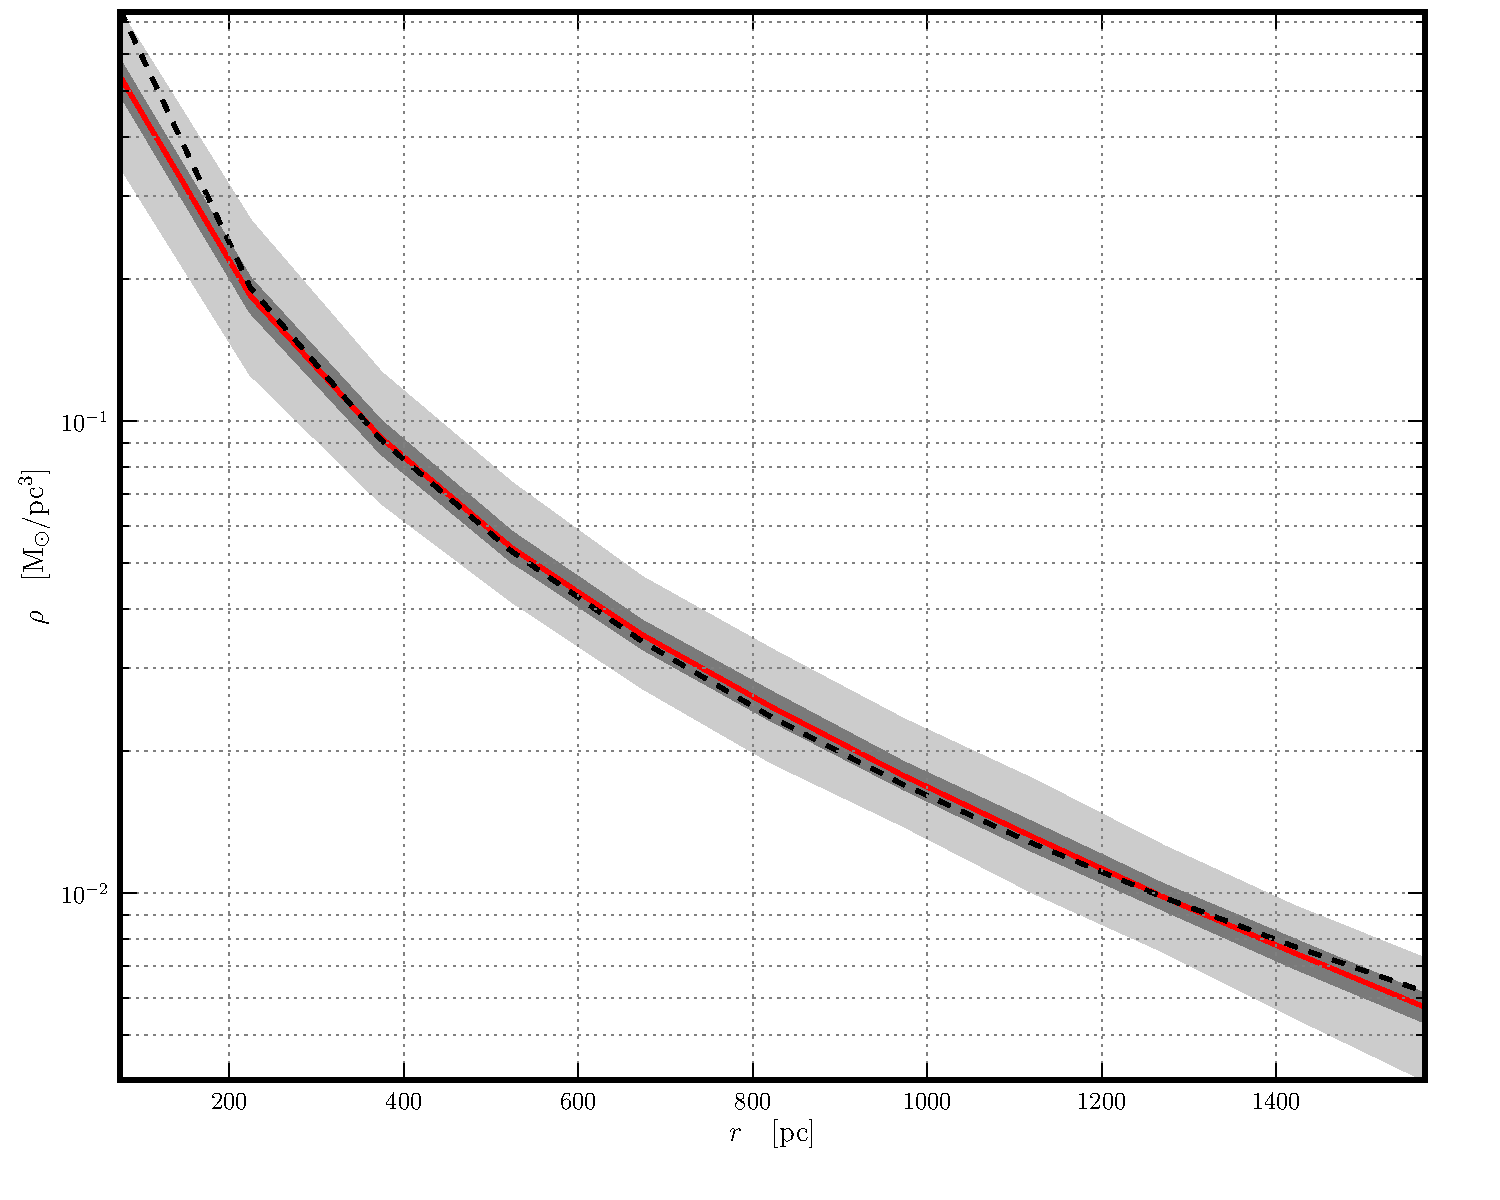
\includegraphics[width=0.5\textwidth]{fig/20130718132442_case_2_10000_0_cprior_nulog_denslog_mslope_rprior_profdens.pdf}
\caption{Reconstructed mass of a cusped model (red shows median,
  shaded areas are 68 and 90 percentiles) for $(2800,4033)$ tracer particles,
  after 50000 iterations. The black dashed curve shows the underlying
  theoretical model.}
\label{fig:cusp}
\end{center}
\end{figure*}

The retrieved models show a distribution with 90 percent certainty
levels (light gray) that encompass the underlying theoretical model
over all radii. For all but the most central bin, the underlying
density profile lies even within $1\sigma$ (dark gray) of all models.

\TODO{d ln rho/d ln r, central density step, constant number of particles / bin}

The errorbars around the scale radius of $1000$ pc of the dark matter
cusp or the scale lengths of $500$ pc or $1000$ pc for the scale radii
of the stellar components are not decreased, thus indicating that the
relative values of the enclosed mass are not better constrained than
at any other radius.





\subsection{Cored Model}
For a cored profile, we have a similar result, see fig. \ref{fig:core}. \TODO{rerun}

\begin{figure*}
\begin{center}
\hspace{-7mm}
%\includegraphics[width=0.5\textwidth]{fig/.pdf}
\caption{A cored profile: Reconstructed mass of the MCMC model (red
  shows median, shaded areas are 68 and 90 percentiles) for $10^4$
  tracer particles after 30000 iterations. The black dashed curve
  shows the underlying theoretical model.}
\label{fig:core}
\end{center}
\end{figure*}

Best restrictions are around $500$pc again, only this time a little
too low.





\subsection{Triaxial mock data}
\TODO{motivation: triaxiality of observed dwarfs, effects from other mass modelling schemes}

The models were generated with a Made 2 Measure algorithm of \cite{Dehnen2009} and are tailored to follow a similar profile to the profiles specified above for the dwarf galaxies. They show a density profile of

\begin{equation}
\rho(r)=\frac{\rho_S}{\left(\frac{r}{r_S}\right)^\gamma\left(1+\left(\frac{r}{r_S}\right)^{1/\alpha}\right)^{\alpha(\beta-\gamma)}}
\end{equation}

with radius $r$, scale radius $r_S=1.5\kpc$, $\alpha=1$,
$\beta=4$. For the cusped profiles we have an inner logarithmic slope
of $-\gamma=-1$, scale density $\rho_S=5.522\cdot 10^7M_\odot/\kpc^3$,
and $M_{\tot}=1.171\cdot10^9M_\odot$, while for the cored one we have
$\gamma=0.23$, $\rho_S=1.177\cdot10^8M_\odot$,
$M_{\tot}=1.802\cdot10^9M_\odot$. The axis ratios are $b/a=0.8$ and
$c/a=0.6$. The stars have negligible mass and follow the same
functional form in the density profile as dark matter, with
$\alpha=0.34, \beta=5.92, \gamma=0.23, r_S=0.81\kpc$.

The velocity anisotropy of the stellar part is calculated via

\begin{equation}
\beta(r)=\frac{r_{s,\beta}^\eta \beta_0+r^\eta \beta_\infty}{r^\eta+r_{s,\beta}^\eta},
\end{equation}

with $r_{s,\beta}=0.81\kpc$, $\beta_0=0$, $\beta_\infty=0.5$ and
$\eta=0.5$, going from isotropic to radially anisotropic with
increasing radius.

\begin{figure*}
\begin{center}
\hspace{-7mm}
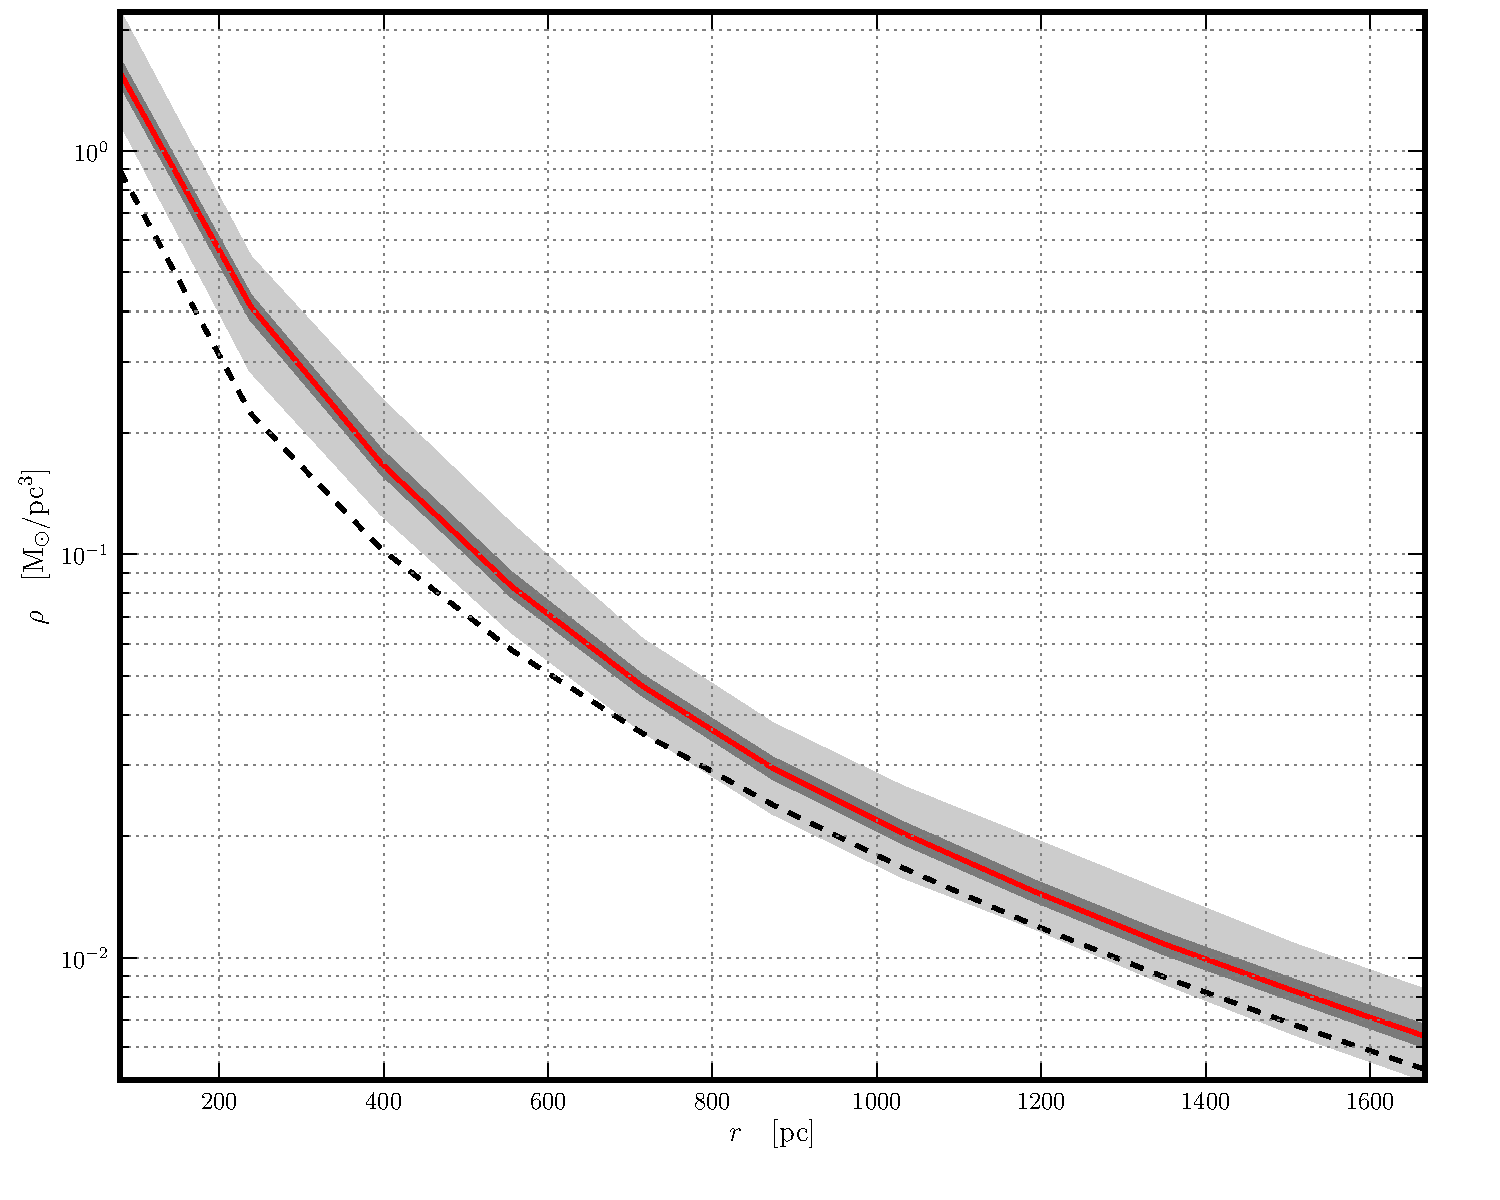
\includegraphics[width=0.5\textwidth]{fig/20130718123300_cprior_nulog_denslog_mslope_rprior_profdens.pdf}
\caption{Density profile of a triaxial mock dwarf, for which the line
  of sight is inclined with 45 degrees with respect to all axes.}
\label{fig:triax}
\end{center}
\end{figure*}

The retrieved density profile (fig. \ref{fig:triax}) is constantly
overestimating the density.

\TODO{other projections}
\TODO{reason: projection}

